\subsection{Dokumentation der Anwendung}
\label{subsec:documentation}

Nachdem wir die Details der Architektur beleuchtet haben, wollen wir die Anwendung des CAD-Viewers aus Benutzersicht dokumentieren.
Die gestartete Anwendung ist standardmäßig unter Port \texttt{8080} erreichbar und stellt sich wie in Screenshot~\ref{fig:app-screenshot} dar.

\begin{figure}[h]
    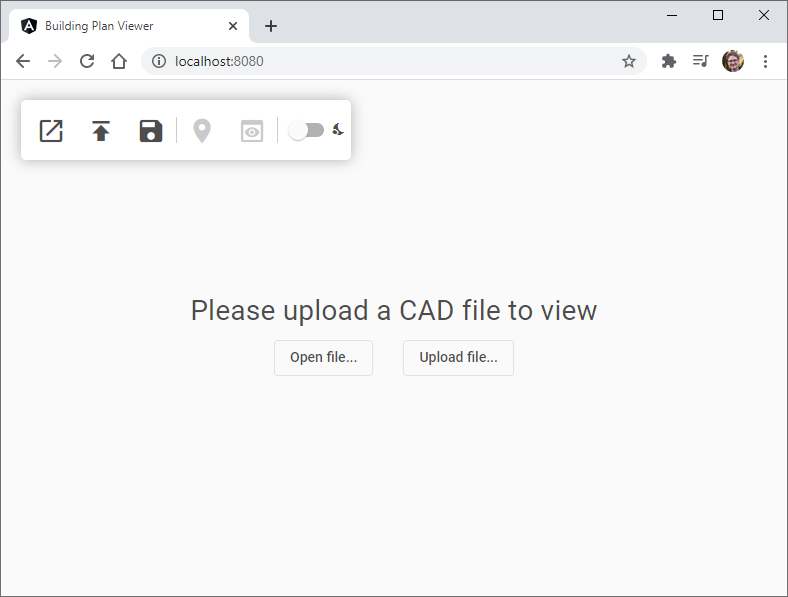
\includegraphics[width=0.5\textwidth]{res/app-screenshot.png}
    \caption{Screenshot der Startansicht der CAD-Viewer Anwendung.}
    \label{fig:app-screenshot}
\end{figure}

In der Grafik ist die Startansicht zu sehen.
Diese umfasst die eigentliche Arbeitsfläche mit einleitenden Aktionen \glqq{}Datei öffnen\grqq{} und \glqq{}Datei hochladen\grqq{} sowie die Steuerungskomponente, welche in jedem Zustand der Webanwendung sichtbar ist.
Die einzelnen Steuerungsmöglichkeiten sind auch nochmal in Abbildung~\ref{fig:controls-component} dargestellt, wobei den einzelnen Icons jeweils eine Zahl zugeordnet ist.

\begin{figure}
    \centering
    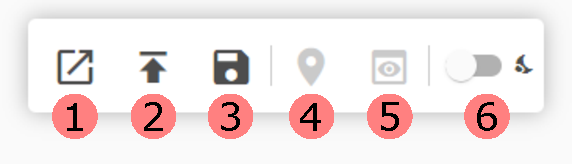
\includegraphics[width=0.3\textwidth]{res/controls.pdf}
    \caption{Steuerungskomponente des Viewer-Programms.}
    \label{fig:controls-component}
\end{figure}

Anhand der Zuordnung beschreiben wir die einzelnen Möglichkeiten:

\begin{enumerate}
    \item \textbf{Datei öffnen}: Der Knopf öffnet einen Dialog zur Auswahl einer CAD-Datei.
    Dabei werden alle bereits hochgeladenen Dateien angezeigt.
    \item \textbf{Datei hochladen}: Ist noch keine CAD-Datei hochgeladen, kann auch keine in der Anwendung dargestellt werden.
    In diesem Fall muss zuerst eine geeignete Datei mit dem Hochladen-Dialog geöffnet werden.
    \item \textbf{Exportieren}: Mit diesem Knopf wird die aktuell gezeichnete CAD-Datei und optional die aktuell ausgewählte Raumzuordnung als HTML Datei exportiert und im Browser heruntergeladen.
    \item \textbf{Raumzuordnungen verwalten}: Der Knopf ist nur aktiviert, wenn eine CAD-Datei geöffnet ist.
    Ist das der Fall, öffnet sich ein Dialog zum Auswählen oder Hochladen von Raumzuordnungen.
    Nach der Auswahl wird die entsprechende Zuordnung über dem Gebäudeplan gezeichnet.
    \item \textbf{Viewport zurücksetzen}: Die Anwendung bietet vielfältige Optionen das Sichtfeld zu manipulieren, sei es durch Zoomen mit dem Mausrad oder dem Verschieben mit der Maus.
    Mit dem Knopf wird das Sichtfeld auf dem Ausgangszustand zurückgesetzt.
    \item \textbf{Wechselknopf helles-/dunkles Thema}: Wechselt das aktuelle Farbschema der Anwendung von Hell zu Dunkel und umgekehrt.
\end{enumerate}

Hat man eine CAD-Datei hochgeladen und über den Auswahldialog ausgewählt, wird der entsprechende Gebäudeplan wie in Screenshot~\ref{fig:app-screenshot-plan} auf der Arbeitsfläche dargestellt.

\begin{figure}
    \includegraphics[width=0.5\textwidth]{res/confidential-example.png}
    \caption{Screenshot eines in der Software gezeichneten Gebäudeplans.}
    \label{fig:app-screenshot-plan}
\end{figure}

Nun bietet der CAD-Viewer zahlreiche Navigationsmöglichkeiten im Gebäudeplan.
So kann die Vergrößerung des Plans über das Mausrad manipuliert werden.
Des Weiteren kann die Arbeitsfläche durch Drücken der linken Maustaste und Ziehen der Maus verschoben werden.
Alternativ ist auch eine Steuerung über die Pfeiltasten der Tastatur möglich.

Ist bereits eine Raumzuordnung hochgeladen worden, kann diese nun über den \glqq{}Raumzuordnungen verwalten\grqq{} Knopf ausgewählt werden.
Alternativ unterstützt der Dialog auch das Hochladen von CSV-Dateien als Raumzuordnung.
Außerdem kann ein Farbschema für die spätere Darstellung auf dem Gebäudeplan ausgewählt werden.

Wir haben in Screenshot~\ref{fig:app-screenshot-mapping} ein Raumzuordnungs-Beispiel dargestellt.
Zur rechten Seite erscheint eine Legende, welche die Kategorien aus dem Clustering-Ergebnis den angezeigten Farben zuordnet.

\begin{figure}
    \includegraphics[width=0.5\textwidth]{res/confidential-example-mapping.png}
    \caption{Screenshot einer Raumzuordnung für einen Gebäudeplan in der Viewer-Anwendung.}
    \label{fig:app-screenshot-mapping}
\end{figure}

\begin{figure}
    \includegraphics[width=0.5\textwidth]{res/confidential-example-tooltip.png}
    \caption{Darstellung eines Tooltips, welcher beim Schweben der Maus über dem Raum erscheinen.}
    \label{fig:app-screenshot-tooltip}
\end{figure}

Lässt der Benutzer den Cursor über die farbig dargestellten Räume schweben, erscheint ein Tooltip mit der Beschreibung der Raumzuordnung.
So können zusätzliche Informationen, wie die Raumfläche in Screenshot~\ref{fig:app-screenshot-tooltip}, angezeigt werden.
Außerdem wird der Raumname des Zuordnungs-Objekts in der Mitte der Räume dargestellt.
